\documentclass[conference]{IEEEtran}
\usepackage{graphicx}
\usepackage{amsmath}
\usepackage{cite}
\usepackage{url}
\usepackage{booktabs}

\begin{document}

\title{Short-Term Ontario Electricity Demand Forecasting Using Machine Learning}

\author{\IEEEauthorblockN{Artem Arutyunov, Nabeegh Khan, Selim Akef}
\IEEEauthorblockA{ECE1513H: Introduction to Machine Learning\\
University of Toronto, Fall 2025}}

\maketitle

\begin{abstract}
Accurate electricity demand forecasting is essential for reliable grid operation and cost optimization in modern power systems. This project develops a machine learning approach to predict short-term hourly electricity demand for Ontario, Canada. We constructed a comprehensive dataset of 109,056 hourly records spanning June 2013 through November 2025, integrating data from four sources: the Independent Electricity System Operator (IESO) for demand data, Environment Canada for hourly weather observations at Toronto Pearson Airport, NASA POWER for satellite-derived solar irradiance, and the Python holidays library for Ontario statutory holiday identification. We engineered 13 additional features including demand lag variables at 1-hour, 24-hour, and 168-hour intervals; cyclical time encodings using sine/cosine transformations; and heating/cooling degree days. We implemented and compared five machine learning models: Linear Regression as a baseline, Support Vector Regression (SVR) with RBF kernel, a Multi-Layer Perceptron Neural Network with three hidden layers, Random Forest with 100 decision trees, and XGBoost with gradient boosting. The Neural Network achieved the best performance with test RMSE of 203.92~MW and $R^2$ of 0.9928, representing a 50.7\% improvement over the linear baseline. Our analysis demonstrates that nonlinear models significantly outperform linear approaches for capturing the complex U-shaped temperature-demand relationship characteristic of Ontario's climate.
\end{abstract}

\begin{IEEEkeywords}
Electricity demand forecasting, machine learning, neural networks, time series prediction, Ontario power grid
\end{IEEEkeywords}

\section{Introduction}

Modern electrical grids face an increasingly complex balancing act between supply and demand. As renewable energy sources expand their share of generation capacity and consumer behavior becomes more variable, the ability to accurately forecast electricity demand has become critical for grid operators worldwide. The consequences of inaccurate predictions are significant and asymmetric: underestimating demand can strain equipment, trigger emergency protocols, and in severe cases cause rolling blackouts affecting millions of customers; overestimating demand leads to costly overgeneration, increased operating reserves, and wasted fuel resources that ultimately raise electricity costs for consumers.

Ontario's electricity system, managed by the Independent Electricity System Operator (IESO)~\cite{ieso}, presents a particularly challenging forecasting environment. The province experiences dramatic seasonal temperature variations---from below $-20^\circ$C during winter cold snaps to above $30^\circ$C during summer heat waves. These temperature extremes create a distinctive U-shaped relationship between temperature and electricity consumption, as illustrated in Fig.~\ref{fig:temp_demand}: demand increases at both cold temperatures (due to electric heating and heat pump operation) and hot temperatures (due to air conditioning loads). This nonlinear pattern fundamentally limits the effectiveness of traditional linear forecasting methods that assume monotonic relationships between predictors and demand.

\begin{figure}[!t]
\centering
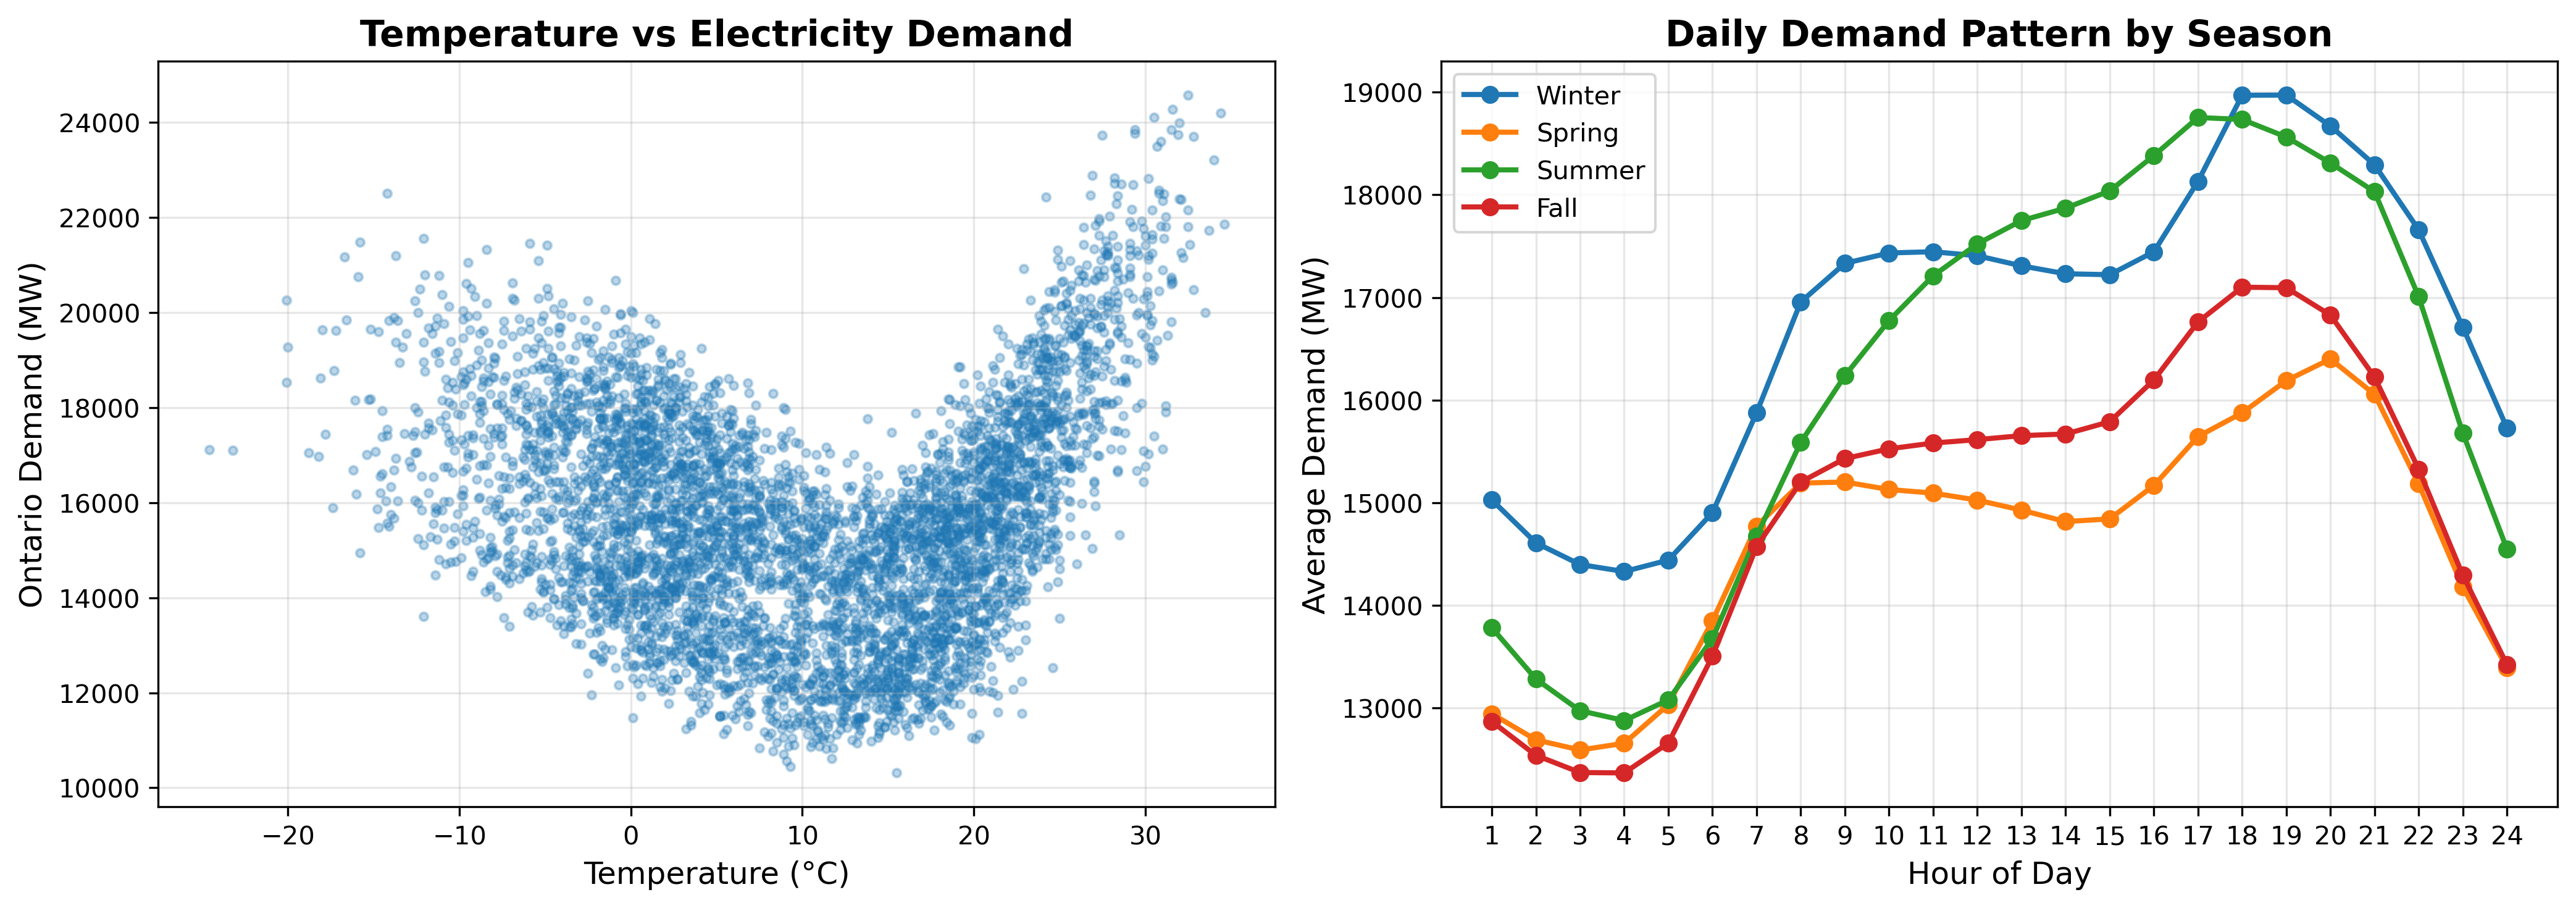
\includegraphics[width=\columnwidth]{temp_demand_seasonal.png}
\caption{Left: U-shaped relationship between temperature and electricity demand in Ontario, showing increased consumption at both temperature extremes due to heating ($<0^\circ$C) and cooling ($>25^\circ$C) loads. Right: Daily demand patterns vary significantly by season, with winter showing highest peak demand around 18:00 and summer exhibiting afternoon peaks driven by air conditioning.}
\label{fig:temp_demand}
\end{figure}

The challenge of electricity demand forecasting has attracted substantial research attention. Traditional approaches rely on statistical time series methods such as ARIMA and exponential smoothing, which capture temporal patterns but struggle with the nonlinear weather-demand relationship. More recent work has applied machine learning techniques including neural networks~\cite{adam}, ensemble methods~\cite{rf,xgboost}, and support vector machines to improve forecast accuracy. However, the optimal model architecture and feature set remain application-specific, depending on local climate patterns, grid characteristics, and data availability.

In this project, we develop a comprehensive machine learning approach to short-term electricity demand forecasting specifically tailored to Ontario's electricity system. We construct a rich multi-source dataset integrating demand records from IESO~\cite{ieso}, weather observations from Environment Canada~\cite{eccc}, solar irradiance from NASA POWER~\cite{nasa}, and calendar information from the Python holidays library~\cite{holidays}. We engineer 13 features designed to capture temporal autocorrelation, nonlinear weather effects, and calendar-based demand patterns. We then implement and rigorously compare five machine learning models spanning the complexity spectrum from simple linear regression to state-of-the-art gradient boosting. Our primary contribution is demonstrating that a properly designed neural network can achieve a 50.7\% reduction in prediction error compared to linear baselines, with practical implications for Ontario grid operation.

\section{System Design}

\subsection{Dataset Assembly and Sources}

We assembled a comprehensive dataset of 109,056 hourly records covering June 2013 through November 2025 from four primary data sources:

\textbf{IESO Electricity Demand~\cite{ieso}:} The target variable---Ontario electricity demand in megawatts (MW)---was obtained from IESO public reports providing hourly system-wide demand measurements. The data spans 12 years with average demand of 15,746~MW, peak demand of 25,450~MW (July 21, 2011 at 3~PM), and minimum demand of 9,831~MW (May 18, 2020 at 3~AM during COVID lockdown).

\textbf{Environment Canada Weather~\cite{eccc}:} Hourly weather observations were collected from Toronto Pearson International Airport (Station ID: 51459), including temperature ($^\circ$C), dew point temperature, relative humidity (\%), wind direction and speed (km/h), visibility (km), and station pressure (kPa). Toronto weather serves as a proxy for Ontario-wide patterns since the Toronto region represents approximately 40\% of Ontario's population and electricity demand.

\textbf{NASA POWER Solar Irradiance~\cite{nasa}:} Satellite-derived solar radiation data was obtained from NASA's Prediction of Worldwide Energy Resources (POWER) API for Toronto coordinates (43.65$^\circ$N, 79.38$^\circ$W). Three parameters were collected: Global Horizontal Irradiance (GHI), Direct Normal Irradiance (DNI), and Diffuse Horizontal Irradiance (DHI), all measured in kWh/m$^2$/day.

\textbf{Ontario Holiday Calendar~\cite{holidays}:} All nine Ontario statutory holidays were generated using the Python holidays library with \texttt{subdiv='ON'} for Ontario-specific observances, including Boxing Day which is statutory only in Ontario.

\subsection{Feature Engineering}

From the raw data sources containing 17 columns, we engineered 13 additional features specifically designed to capture the complex dynamics driving electricity consumption patterns, resulting in 31 total features for modeling:

\textbf{Lag Features (5):} Recognizing that electricity consumption exhibits strong temporal autocorrelation---demand at any hour is highly correlated with recent demand---we created lag features at three intervals. \texttt{Demand\_Lag\_1h} captures short-term momentum, \texttt{Demand\_Lag\_24h} captures daily periodicity, and \texttt{Demand\_Lag\_168h} (one week) captures weekly patterns such as weekday versus weekend differences. Additionally, we computed \texttt{Demand\_RollingAvg\_24h} and \texttt{Demand\_RollingAvg\_168h} rolling averages to smooth noise while preserving trends.

\textbf{Degree Days (2):} Using the standard base temperature of $18^\circ$C, we calculated Heating Degree Days as $\text{HDD} = \max(18 - T, 0)$ and Cooling Degree Days as $\text{CDD} = \max(T - 18, 0)$, which are industry-standard metrics quantifying heating and cooling requirements.

\textbf{Temperature Transformations (2):} To model the U-shaped temperature-demand relationship shown in Fig.~\ref{fig:temp_demand}, we created \texttt{Temp\_x\_Hour} (temperature $\times$ hour interaction capturing time-varying HVAC effects) and \texttt{Temp\_Squared} ($T^2$, allowing models to capture the parabolic relationship where demand increases at both temperature extremes).

\textbf{Cyclical Encodings (4):} Rather than treating hour-of-day and month-of-year as linear or categorical variables, we applied sine and cosine transformations: $\sin(2\pi \cdot \text{hour}/24)$, $\cos(2\pi \cdot \text{hour}/24)$, $\sin(2\pi \cdot \text{month}/12)$, and $\cos(2\pi \cdot \text{month}/12)$. This encoding ensures the model understands that hour 23 and hour 0 are temporally adjacent (not 23 units apart), and similarly that December and January represent continuous seasonal progression.

After dropping 168 rows with missing lag features (the initial hours where historical lags are unavailable), our final modeling dataset contained 108,888 samples with 31 features. Remaining missing values in HOEP prices and solar irradiance were handled via forward-fill then backward-fill imputation.

\subsection{Model Selection and Alternatives}

Following the course project requirement to demonstrate an improvement process starting from concepts discussed in lectures and extending to methods beyond the course, we implemented five models representing a spectrum of complexity:

\textbf{Linear Regression} (Course Concept, Lecture 3): We implemented ordinary least squares linear regression using scikit-learn~\cite{sklearn} as our baseline model. Linear regression provides an interpretable, computationally efficient solution that serves as the reference point for measuring improvement. However, it fundamentally cannot capture the nonlinear temperature-demand relationship or complex feature interactions.

\textbf{Support Vector Regression with RBF Kernel} (Course Concept, Lectures 5--6): Building on the SVM concepts covered in lectures, we applied SVR with a radial basis function kernel: \texttt{SVR(kernel='rbf', C=100, gamma='scale', epsilon=0.1, cache\_size=1000)}. The RBF kernel maps features to a high-dimensional space where nonlinear relationships become linear. However, SVR has computational complexity of $O(n^2)$ to $O(n^3)$ for training, which becomes prohibitive with our 83,000+ training samples.

\textbf{Multi-Layer Perceptron Neural Network} (Extended from Lecture 8): Extending the neural network concepts from Lecture 8, we designed a feedforward architecture using scikit-learn's \texttt{MLPRegressor} with three hidden layers containing 128, 64, and 32 neurons respectively. Each hidden layer uses ReLU activation. Key hyperparameters include: Adam optimizer~\cite{adam} with adaptive learning rate (initial value 0.001), L2 regularization with $\alpha=0.0001$ to prevent overfitting, early stopping with patience of 10 epochs monitoring validation loss, maximum 200 iterations, and random state 42 for reproducibility.

\textbf{Random Forest} (Beyond Course): Random Forest~\cite{rf} is an ensemble method that constructs multiple decision trees during training and outputs the average prediction. We configured: \texttt{n\_estimators=100} trees, \texttt{max\_depth=20}, \texttt{min\_samples\_split=5}, \texttt{min\_samples\_leaf=2}, \texttt{max\_features='sqrt'}, and parallel processing with \texttt{n\_jobs=-1}.

\textbf{XGBoost} (Beyond Course): Extreme Gradient Boosting~\cite{xgboost} represents state-of-the-art gradient boosting, building trees sequentially where each tree corrects errors of previous trees. Configuration: \texttt{n\_estimators=200} boosting rounds, \texttt{max\_depth=8}, \texttt{learning\_rate=0.1}, \texttt{subsample=0.8}, \texttt{colsample\_bytree=0.8}, L1 regularization \texttt{reg\_alpha=0.1}, L2 regularization \texttt{reg\_lambda=1.0}, and histogram-based tree method for efficiency.

\subsection{Data Splitting and Preprocessing}

The complete dataset was split chronologically to prevent future information leakage: 77\% training (83,843 samples), 8\% validation (8,711 samples), and 15\% test (16,334 samples). For models requiring standardized inputs (Neural Network, SVR), all features were normalized using z-score standardization (subtracting mean, dividing by standard deviation) computed on the training set only, then applied identically to validation and test sets. Random Forest and XGBoost do not require feature scaling due to their tree-based splitting mechanisms.

\section{Results}

We evaluate all models using four complementary metrics: Root Mean Square Error (RMSE) measuring prediction accuracy in MW, coefficient of determination ($R^2$) indicating proportion of variance explained, Mean Absolute Error (MAE) providing average error magnitude, and Mean Absolute Percentage Error (MAPE) expressing errors as percentages. Table~\ref{tab:results} presents the comprehensive performance comparison, with visual rankings shown in Fig.~\ref{fig:rmse_ranking}.

\begin{table}[!t]
\centering
\caption{Model Performance Comparison on Test Set}
\label{tab:results}
\begin{tabular}{lccccc}
\toprule
\textbf{Model} & \textbf{RMSE} & \textbf{$R^2$} & \textbf{MAE} & \textbf{MAPE} & \textbf{Time} \\
 & (MW) & & (MW) & (\%) & (s) \\
\midrule
Neural Network & \textbf{203.92} & \textbf{0.9928} & \textbf{156.74} & \textbf{0.97} & 185.1 \\
XGBoost & 222.86 & 0.9914 & 160.11 & 0.97 & 2.7 \\
Random Forest & 321.30 & 0.9821 & 237.60 & 1.43 & 6.9 \\
Linear Regression & 413.25 & 0.9704 & 315.26 & 1.94 & 0.5 \\
SVR (RBF) & 476.05 & 0.9607 & 301.70 & 1.73 & 570.2 \\
\bottomrule
\end{tabular}
\end{table}

\begin{figure}[!t]
\centering
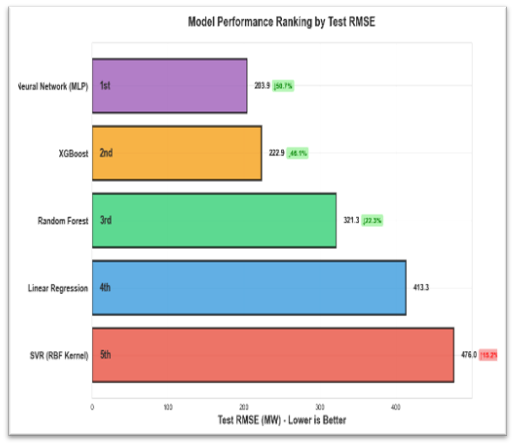
\includegraphics[width=\columnwidth]{rmse_ranking.png}
\caption{Model performance ranking by test RMSE. The Neural Network achieves the best performance (203.9~MW, 50.7\% improvement over baseline), followed closely by XGBoost (222.9~MW, 46.1\% improvement). SVR performs worst despite its nonlinear capability, showing 15.2\% degradation versus Linear Regression.}
\label{fig:rmse_ranking}
\end{figure}

The Neural Network achieves the lowest test RMSE at 203.92~MW, representing a \textbf{50.7\% improvement} over the Linear Regression baseline of 413.25~MW. This substantial error reduction demonstrates the value of capturing nonlinear patterns that linear models cannot represent. The network converged at iteration 102 based on early stopping. XGBoost~\cite{xgboost} performs nearly as well with RMSE of 222.86~MW (46.1\% improvement) while requiring only 2.7 seconds of training time compared to 185 seconds for the Neural Network---making it highly attractive for operational deployment where models may require frequent retraining.

Random Forest~\cite{rf} achieves 22.3\% improvement over baseline with RMSE of 321.30~MW, demonstrating that ensemble tree methods capture meaningful nonlinear structure even without the sequential error correction of boosting. However, its accuracy falls substantially short of both the Neural Network and XGBoost.

Most notably, SVR performs \textit{worse} than Linear Regression despite its theoretical ability to capture nonlinear relationships through the kernel trick. With test RMSE of 476.05~MW compared to 413.25~MW for Linear Regression, SVR shows a 15.2\% degradation in performance. This counterintuitive result stems from kernel methods' computational complexity: with $O(n^2)$ to $O(n^3)$ scaling, the 83,843-sample training set overwhelms SVR's quadratic programming optimization. Even after 570 seconds of training (1140$\times$ slower than Linear Regression), the optimizer produces a suboptimal solution. This finding illustrates that sophisticated algorithms do not automatically outperform simpler approaches---computational tractability matters critically at scale.

\begin{figure}[!t]
\centering
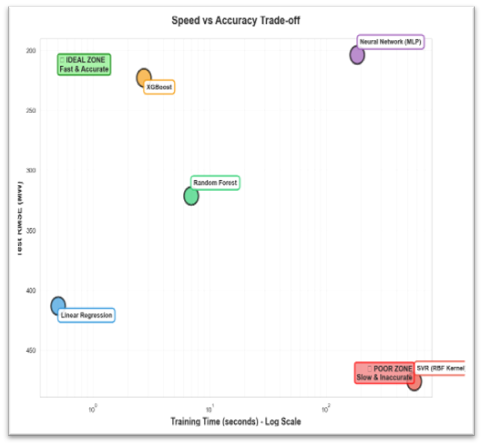
\includegraphics[width=\columnwidth]{speed_accuracy.png}
\caption{Speed versus accuracy trade-off (log scale for training time). XGBoost occupies the ideal zone: fast training (2.7s) with excellent accuracy (222.9~MW RMSE). SVR occupies the worst position---slow (570s) and inaccurate (476~MW). The Neural Network achieves best accuracy but requires 68$\times$ longer training than XGBoost.}
\label{fig:speed_accuracy}
\end{figure}

Fig.~\ref{fig:speed_accuracy} visualizes the critical speed-accuracy trade-off. XGBoost occupies an ideal position: fast training (2.7s) combined with excellent accuracy (222.86~MW RMSE). For operational forecasting systems requiring frequent updates, XGBoost may be preferred despite the Neural Network's slight accuracy advantage. SVR occupies the worst quadrant---both slow and inaccurate---demonstrating that kernel methods scale poorly to datasets of this size.

\begin{figure}[!t]
\centering
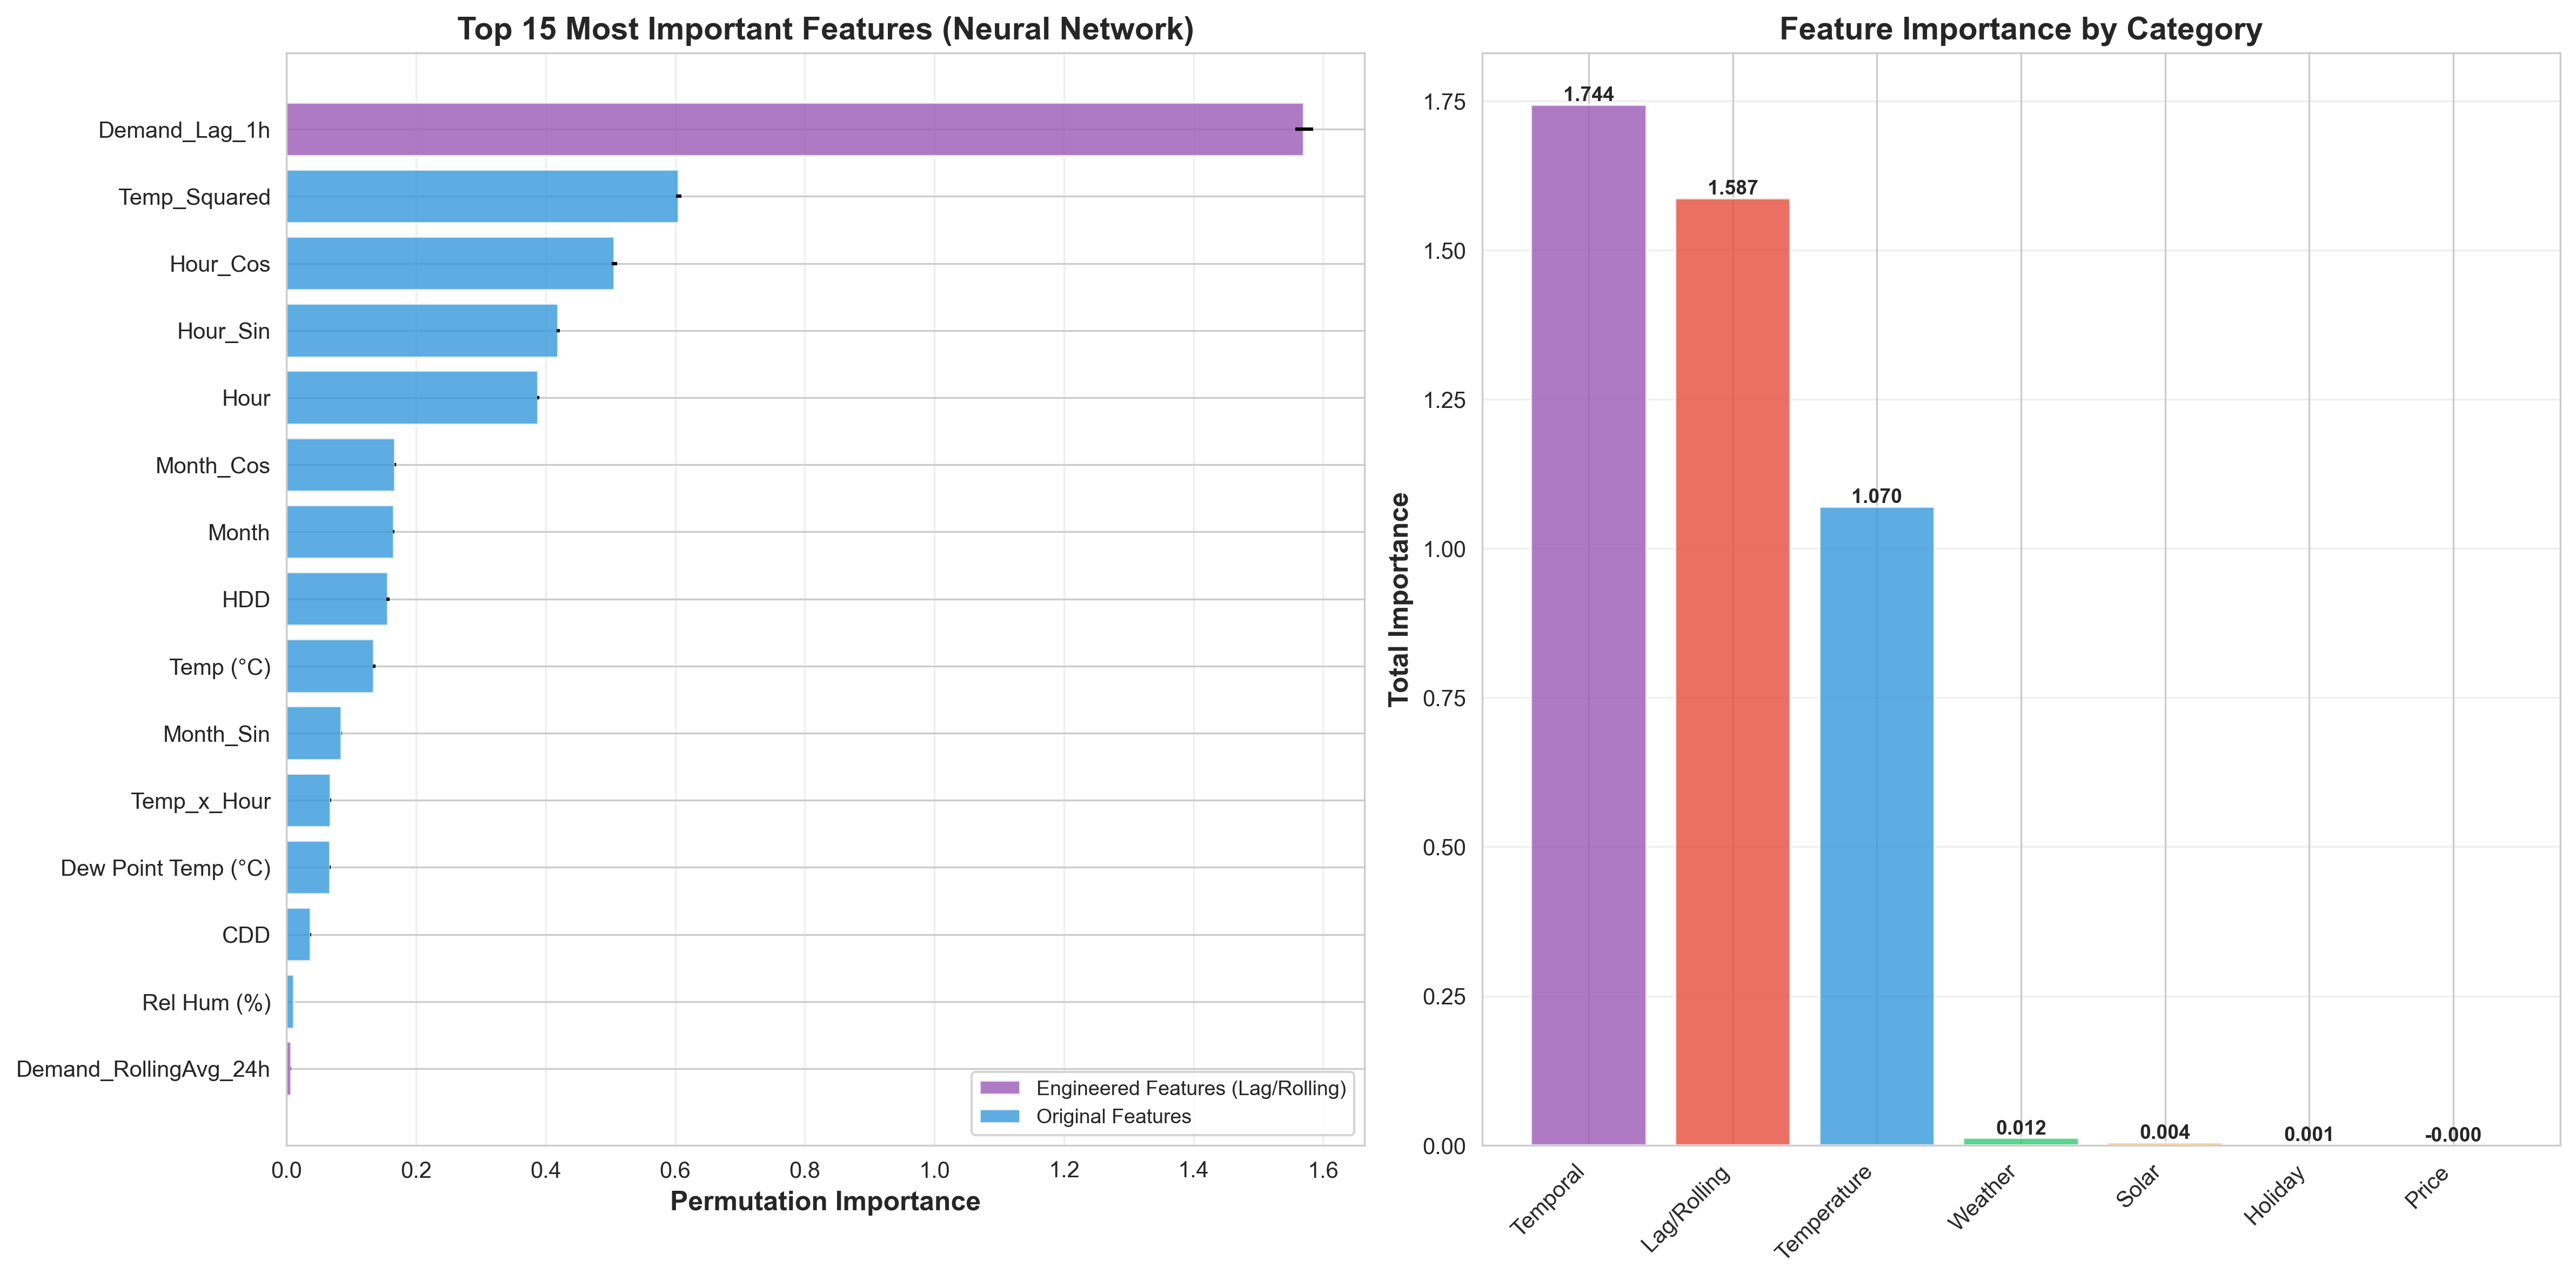
\includegraphics[width=\columnwidth]{feature_importance.png}
\caption{Feature importance analysis using permutation importance. Left: Top 15 features ranked by importance, with \texttt{Demand\_Lag\_1h} dominating (1.587), followed by \texttt{Temp\_Squared} (0.55) validating the U-shaped hypothesis. Right: Importance aggregated by category showing temporal (1.744) and lag features (1.587) contribute most, while weather variables contribute minimally (0.012).}
\label{fig:features}
\end{figure}

Feature importance analysis using permutation importance on the Neural Network (Fig.~\ref{fig:features}) reveals that \texttt{Demand\_Lag\_1h} dominates all other features with importance score of 1.587, confirming that electricity demand exhibits strong temporal autocorrelation---the best predictor of current demand is recent demand. \texttt{Temp\_Squared} ranks second (0.55), validating our hypothesis about the nonlinear temperature-demand relationship and justifying the quadratic temperature transformation. Cyclical hour encodings (\texttt{Hour\_Cos}: 0.45, \texttt{Hour\_Sin}: 0.35) effectively capture the predictable daily demand pattern visible in Fig.~\ref{fig:temp_demand}. By category, temporal features contribute 1.744 total importance, lag/rolling features contribute 1.587, and temperature features contribute 1.070, while weather variables (humidity, pressure, wind) contribute only 0.012---suggesting that temperature dominates other atmospheric effects for demand prediction.

The Neural Network's error distribution is approximately Gaussian with mean $-22.92$~MW and standard deviation 202.64~MW, indicating the model has no systematic bias toward over- or under-prediction. The small negative mean suggests very slight under-prediction on average, but this is negligible relative to the typical demand magnitude of 15,000+~MW.

\section{Concluding Remarks}

This project demonstrates that machine learning provides substantial improvements for electricity demand forecasting in Ontario's power system. Our Neural Network model achieves 50.7\% RMSE reduction compared to linear regression, with $R^2$ of 0.9928 explaining over 99\% of hourly demand variance. The success stems from three key factors: comprehensive multi-source data integration combining demand from IESO, weather from Environment Canada, solar irradiance from NASA POWER, and holidays; thoughtful feature engineering that captures temporal autocorrelation through lag variables and nonlinear weather effects through temperature transformations and cyclical encodings; and appropriate model selection matching algorithmic complexity to underlying data patterns.

The comparison of five models yields important practical insights. While the Neural Network achieves the best accuracy, XGBoost~\cite{xgboost} provides a compelling alternative with 46.1\% improvement and 68$\times$ faster training (2.7s vs 185s)---valuable for operational systems requiring frequent model updates. Conversely, SVR's poor performance demonstrates that sophisticated algorithms do not automatically outperform simpler approaches; the $O(n^2)$ kernel computation becomes a liability rather than an asset at this data scale with 83,000+ training samples.

Future work could extend this approach by incorporating real-time electricity price signals as features since price-responsive loads affect demand patterns, investigating attention-based neural architectures such as Transformers for longer-horizon multi-step forecasting, and deploying the model in an operational setting with automated rolling retraining to adapt to evolving consumption patterns and climate trends.

\begin{thebibliography}{8}

\bibitem{ieso}
Independent Electricity System Operator (IESO), ``Data Directory,'' 2025. [Online]. Available: https://www.ieso.ca/en/Power-Data/Data-Directory

\bibitem{eccc}
Environment and Climate Change Canada, ``Historical Climate Data,'' 2025. [Online]. Available: https://climate.weather.gc.ca/

\bibitem{nasa}
NASA Langley Research Center, ``POWER Data Access Viewer,'' 2025. [Online]. Available: https://power.larc.nasa.gov/

\bibitem{adam}
D. P. Kingma and J. Ba, ``Adam: A Method for Stochastic Optimization,'' in \textit{Proc. Int. Conf. Learning Representations (ICLR)}, 2015.

\bibitem{xgboost}
T. Chen and C. Guestrin, ``XGBoost: A Scalable Tree Boosting System,'' in \textit{Proc. ACM SIGKDD Int. Conf. Knowledge Discovery and Data Mining}, 2016, pp. 785--794.

\bibitem{rf}
L. Breiman, ``Random Forests,'' \textit{Machine Learning}, vol. 45, no. 1, pp. 5--32, 2001.

\bibitem{sklearn}
F. Pedregosa \textit{et al.}, ``Scikit-learn: Machine Learning in Python,'' \textit{J. Mach. Learn. Res.}, vol. 12, pp. 2825--2830, 2011.

\bibitem{holidays}
Python Software Foundation, ``holidays: Generate and work with holidays in Python,'' 2025. [Online]. Available: https://pypi.org/project/holidays/

\end{thebibliography}

\end{document}
